\chapter{Methode}\label{chap:m} Die Methode dieser Untersuchung besteht darin,
die in der Fragestellung beschriebene künstliche Intelligenz (KI) zu entwickeln
und dessen Leistung auszuwerten (siehe \doubleref{chap:m_auswert}). Die
Diskussion dieser Resultate führt schlussendlich zu einer Antwort auf die
Fragestellung. Die Entwicklung der KI besteht aus zwei Teilen. Der eine Teil
umfasst die Definition der Kriterien, nach denen die Leistung der KI evaluiert
wird (siehe \doubleref{chap:m_eval}). Der andere Teil umfasst die Entwicklung
der KI. Dazu gehört die Entwicklung einer grundlegenden Architektur (siehe
\doubleref{chap:m_grund}), sowie die Vollendung der KI mit verschiedenen
Variationen und Ansätzen (siehe \doubleref{chap:m_var}). Die Variationen sind
dabei Versuche, die Leistung der KI zu maximieren oder ihr Verhalten zu
verändern. Ein spezielle Variation, die sich dabei von der ursprünglichen
Absicht entfernt, ist die Umwandlung in eine generative KI, die nicht mehr
Nachzechnet und stattdessen eigene Zeichnungen ohne Vorlage kreiert (siehe
\doubleref{chap:m_generativ}).


\section{Grundprogramm}\label{chap:m_grund} Das Grundprogramm ist eine flexibel
anwendbare Architektur der KI, die als Grundlage für eine Vielzahl an
Variationen dient. Das Grundprogramm bietet dabei eine Trainingsumgebung für die
KI, eine Zeichenumgebung und das Reinforcement Learning Modell (Deep
Q-Learning), zusammen mit dem Agent und dem neuronalen Netz (siehe
\doubleref{sub:t_rl_func}). Das Grundprogramm beinhaltet dabei keine
Reward-Function und ist somit keine funktionale Version der KI.
Das Grundprogramm ist in Python unter der Verwendung des Keras
Frameworks implementiert (siehe \doubleref{chap:t_ml}).


\subsection{Doodle-SDQ als Basis}\label{sub:m_grund_dood} Das Reinforcement
Learning Modell des Grundprogramms basiert auf Doodle-SDQ (siehe
\doubleref{sub:t_ver_dood}). Von Doodle-SDQ ist das neuronale Netz, bezogen auf
die Form des Inputs, des Outputs und den Hidden Layers, grösstenteils
übernommen. Die relevanten Anpassungen zwischen Doodle-SDQ und dem Grundprogramm
dieser Arbeit sind nachfolgend erläutert.
 
Bei der Umgebung handelt es sich, wie bei Doodle-SDQ, um eine Zeichenfläche,
worauf sich der Agent bewegt. Das Grundprogramm wird auf das
Nachzeichnen von Ziffern trainiert. Die Ziffern stammen aus dem MNIST Datenset
(siehe \doubleref{chap:t_ml}) und haben somit eine Grösse von $28\times28$
Pixeln. Die Fläche, worauf sich der Agent bewegen  
kann, hat folglich auch eine Grösse von $28\times28$ Pixeln. Der Global Stream
(siehe \doubleref{sub:t_ver_dood}) des Inputs in das neuronale Netz ändert sich
bis auf die neue Grösse der Bilder nicht. Die Pixel der Bilder, wie auch die
Zeichenfläche, nehmen den Wert von einem Bit an. Eine Null repräsentiert einen
schwarzen (nicht gezeichneten) Pixel an dieser Stelle im Bild und eine Eins
einen weissen (gezeichneten) Pixel. Die genaue Architektur des neuronalen Netzes
ist in der folgenden Abbildung angegeben (siehe \autoref{fig:architecture}). 
 
%Bild architecture
\begin{figure}[!ht]
 \centering
 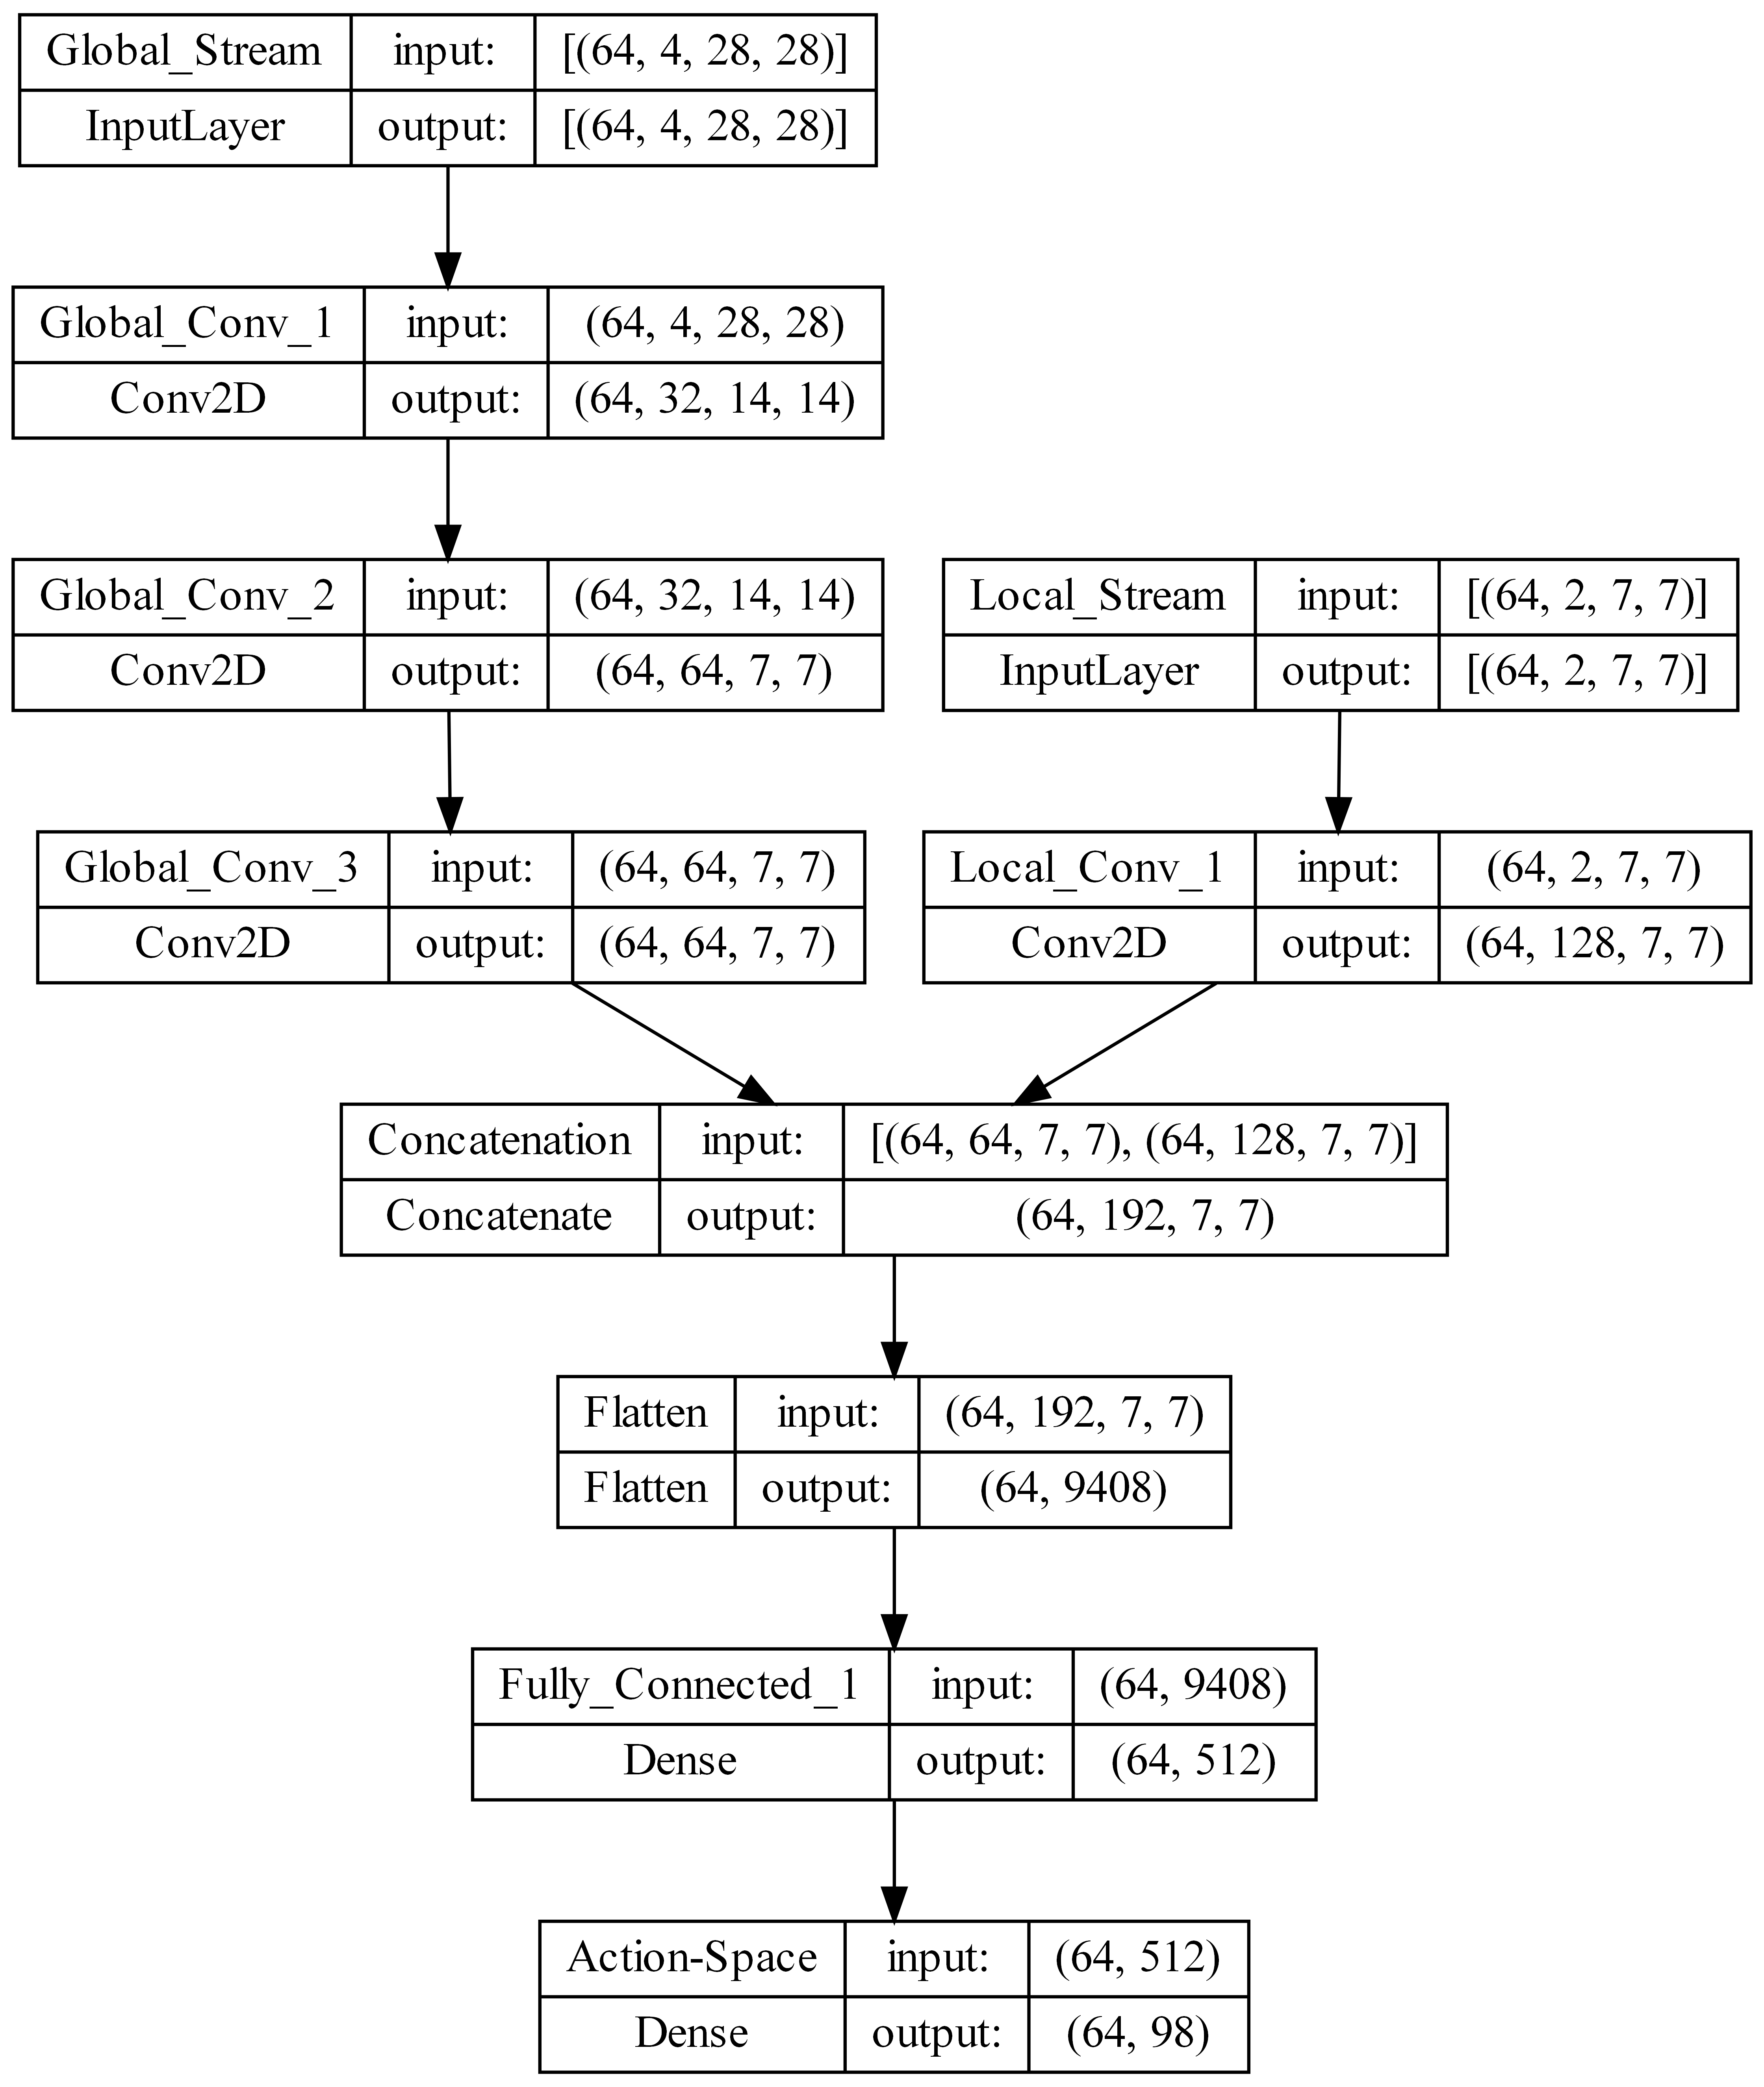
\includegraphics[width=\textwidth-4cm]{images/methode/architecture.png}
 \caption{Architektur des neuronalen Netzes im Grundprogramm (eigene Abbildung, mit Keras erstellt). Jeder Block repräsentiert einen Layer. Die Form des Inputs und des Outputs ist von jedem Layer angegeben}\label{fig:architecture}
\end{figure}
 
Der Local Stream und damit auch der Local image Patch schrumpfen von $11\times11$
Pixel auf $7\times7$ Pixel. Somit schrumpft gleichzeitig der Action-Space (siehe
\doubleref{sub:t_rl_func}) des Agenten von $2\cdot11\cdot11 = 242$ Actions auf
$2\cdot7\cdot7 = 98$ Actions. Das bedeutet für den Agent, dass er sich pro Step
um maximal drei Pixel von seiner Position wegbewegen kann. Diese Bewegung kann
der Agent entweder zeichnend oder nicht zeichnend ausführen (siehe
\autoref{fig:actionspace}).
 
%bild normal actionspace
\begin{figure}[!ht]
 \centering
 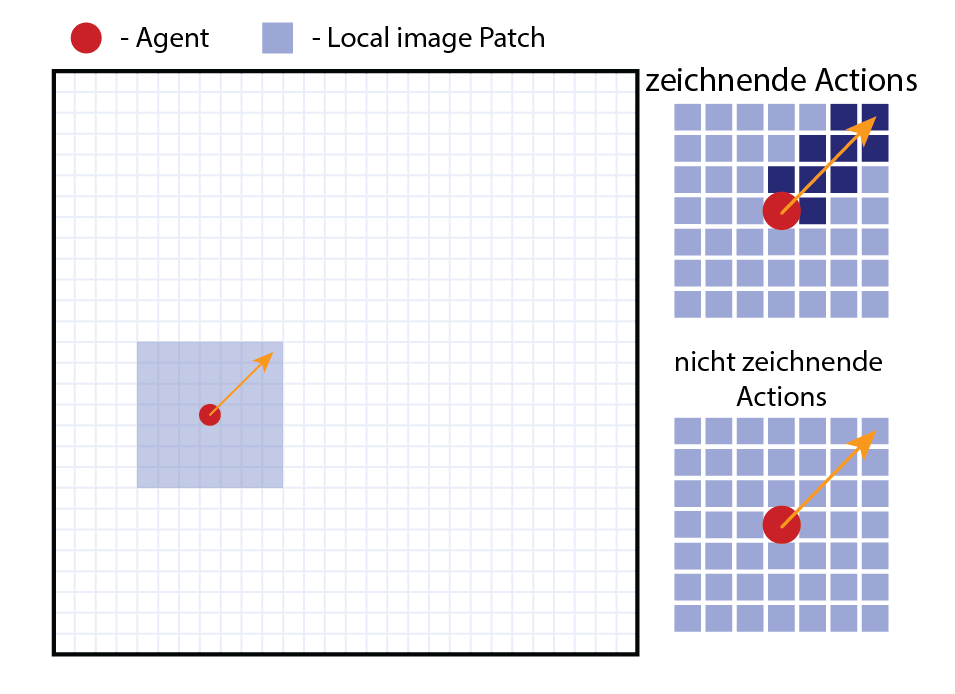
\includegraphics[width=\textwidth]{images/methode/actionspace.png}
 \caption{Action-Space im Grundprogramm}\label{fig:actionspace}
\end{figure}
 
Falls der Agent die Action zeichnend ausführt, zieht das Programm einen Strich
zwischen der alten und der neuen Position. Das bedeutet, dass alle Pixel
der Zeichenfläche zwischen den beiden Positionen weiss werden. Der Strich hat eine
festgelegte Breite von $3$ Pixeln. Am Anfang jeder Episode, also mit jeder neuen
Ziffer, startet der Agent in einer zufälligen Position im nicht zeichnenden
Zustand. Am Anfang jeder Episode ist die Zeichenfläche leer, also vollkommen
Schwarz.

Das Grundprogramm verwendet als Policy für die Wahl der Actions standardmässig
Epsilon-Greedy. Die Softmax Policy ist allerdings auch implementiert und nach
belieben verwendbar.


\subsection{Erweiterungen}\label{sub:m_grund_erweiterungen} Die folgenden
Eigenschaften des Grundprogramms sind Erweiterungen der Architektur von
Doodle-SDQ.

Die erste Erweiterung beschreibt die behandlung von illegalen Actions. Alle
Actions, die den Agent über die vorgegebene Zeichenfläche hinaus positionieren
würden, sind nicht zulässig. Diese Actions sind für den Agent nicht wählbar
und ihr optimaler Q-Value (siehe \doubleref{sub:t_rl_func}) ist in jedem Fall
$0$. Das hat zur Folge, dass nach dem Training die allermeisten unzulässigen
Actions einen Q-Value nahe oder gleich $0$ haben. Das senkt die
Wahrscheinlichkeit, dass der Agent versucht, eine unzulässige Action
auszuführen.

Die zweite Erweiterung betrifft den Action-Space mit der Einführung einer Stopp
Action. Wenn der Agent diese Action wählt, bricht die Zeichnung ab. Der Agent
kann somit frei entscheiden, wann die Zeichnung fertig ist. Die Stopp Action
kann während dem Training dem Agent verboten werden. In diesem Fall wird die
Action als unzulässig behandelt.

 
\subsection{Präparierung der Daten und Optimierung}\label{sub:m_grund_data}
Die Trainingsdaten bestehen aus $36'000$ Bildern von handgeschriebenen Ziffern
aus dem MNIST Datenset (siehe \doubleref{chap:t_ml}). Die restlichen Bilder des
MNIST Datensets machen die Testdaten aus. Die Bilder im Datenset sind als Bitmap
dargestellt, wobei jedes Element (jeder Pixel) einen Wert zwischen $0$ und $255$
annimmt. Die Zahl repräsentiert eine Graustufe, wobei $0$ Schwarz ist und $255$
Weiss. Diese Graustufen werden entfernt. Jeder Pixel mit einem Wert über $0$
übernimmt den Wert $1$, wodurch die Bilder nur noch aus Einsen und Nullen
bestehen. Dabei ist $0$ Schwarz und $1$ Weiss (siehe \autoref{fig:norm-v-nogray}).
So stimmen die Bilder mit den Zeichnungen, die der Agent produzieren kann,
überein.
 
%Bild normal num vs nogray num
\begin{figure}[!ht]
 \centering
 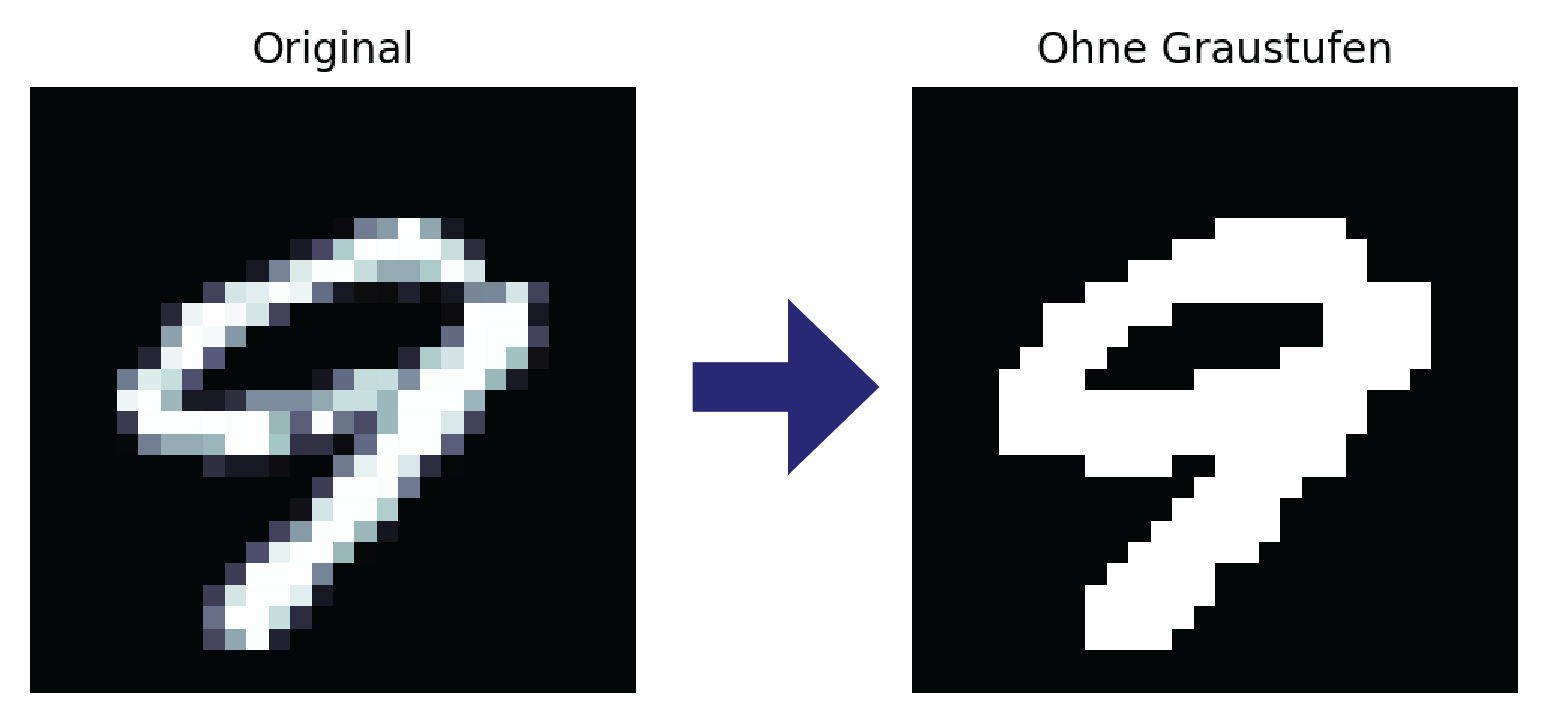
\includegraphics[width=\textwidth]{images/methode/norm-v-nogray.png}
 \caption{Entfernung der Graustufen im MNIST Datenset. (eigene Abbildung)}\label{fig:norm-v-nogray}
\end{figure}
 
 
Das Grundprogramm trainiert mit $5'000$ Bildern, von denen jede Ziffer $500$
Bilder ausmacht. Die restlichen Bilder in den Trainingsdaten sind für mögliche 
Erweiterungen aufgehoben. Der Agent zeichnet jedes der $5'000$ Bilder ein Mal und
trainiert somit für $5'000$ Episodes. Der Agent zeichnet für $64$ Steps pro
Episode, falls die Stopp Action nicht früher gewählt wird.
 
Die Hyperparameter aller Versionen der KI sind durch den Bayesian Optimization
Algorithmus optimiert (siehe \doubleref{sub:t_ml_hyper}). Die Implementierung
des Algorithmus in Python stammt von \cite{fernando_nogueira_bayesian_2014}. Der
Algorithmus ändert sich für verschiedene Variationen der KI nicht und ist somit
Teil des Grundprogramms. Mit jeder Iteration des Baysian Optimization
Algorithmus trainiert das Reinforcement Learning Modell für eine vom Algorithmus
selbst bestimmte Anzahl Episodes. Die Zielvariable, die durch den Baysian
Optimization Algorithmus maximiert werden soll, wird am Ende jeder Iteration des
Trainings in der Testumgebung berechnet (siehe \doubleref{sub:m_auswert_test}).
Unter welchem Kriterium (siehe \doubleref{chap:m_eval}) der Wert der
Zielvariable berechnet wird ist frei wählbar  
basiert, ist frei wählbar.
 
\section{Evaluation der Leistung}\label{chap:m_eval}
In diesem Unterkapitel sind die Kriterien definiert, welche die Leistung der
künstlichen Intelligenz evaluieren. Spezifischer beschreiben die
Kriterien, wie gut die KI nachzeichnet. Für eine präzise und objektive
Evaluation sind alle Kriterien durch einen Zahlenwert repräsentiert. Die
Kriterien und ihre jeweilige Berechnung werden nachfolgend beschrieben.
 
\subsection{Erkennbarkeit}\label{sub:m_eval_rec}
Das Kriterium der Erkennbarkeit beschreibt, ob in der Vorlage das gleiche Motiv
wie in der Zeichnung der künstlichen Intelligenz erkannt wird. Wenn
Beispielsweise in beiden Fällen eine Fünf erkannt wird, hat das Kriterium den
Wert $1$. Wird in der Vorlage eine Fünf erkannt, aber in der Zeichnung eine
Vier, hat das Kriterium den Wert $0$
 
Das erkannte Motiv wird durch eine zweite KI beurteilt (siehe
\doubleref{sub:t_ml_func}). Diese klassifizierden Machine Learning Modelle sind
spezifisch auf Bilder ohne Graustufen trainiert, welche die nachzeichnende KI
dieser Arbeit produzieren kann. Der Output Layer der klassifiziernden KI hat
Softmax mit einer hohen Temperatur als Activation Function (siehe
\doubleref{chap:t_ml}). Das versichert, dass die KI nur eine eindeutige
Klassifizierung trifft wenn die Wahrscheinlichkeit für dessen Richtigkeit hoch
ist. Für die verschiedenen Arten von Strichbildern, welche die KI zeichnen soll,
werden spezifische klassifizierende Machine Learning Modelle mit den zugehörigen
Datensets trainiert. Diese Modelle, zusammen mit ihrer Genauigkeit, sind in der
folgenden Tabelle (siehe \autoref{tab:models}) aufgeführt. Das Neuronale Netz
der Modelle stammt aus einem online Machine Learning Kurs \cite{wang_deep_2021}. %Todo Quelle Online Modelle

\begin{table}[!ht]
 \centering  
 \begin{tabular}{|l|l|l|l|}
 \hline
     Art & Trainiert mit & Genauigkeit [\%]\\ \hline
     Ziffern & MNIST & 99\\ \hline
     Buchstaben  & EMNIST Letters & 91\\ \hline
     \makecell{Strichbilder\\von Objekten}  & Auswahl aus QuickDraw & 98\\ \hline
 \end{tabular}
 \caption{Vortrainierte Modelle}\label{tab:models}
\end{table}
 
\subsection{Prozentuale Übereinstimmung}\label{sub:m_eval_proc}
Dieses Kriterium beschreibt die prozentuale Übereinstimmung der weissen
(gezeichneten) Pixel zwischen der Vorlage und der Zeichnung der KI (siehe
\doubleref{chap:m_grund}). Der Wert $K$ dieses Kriteriums zu dem Step $t$
berechnet sich aus folgender Formel:
\[ K(t) = \frac{G(t)}{G_{\max}} \] $G_{\max}$ entspricht der Anzahl aller
weissen Pixeln in der Vorlage. $G(t)$ entspricht der Anzahl der weissen Pixel,
die zwischen der Vorlage und der Zeichenfläche übereinstimmen. Die Pixel, die
nicht übereinstimmen, zählen negativ für $G(t)$. $G(t)$ und somit auch $K(t)$
können dadurch auch negative Werte annehmen. Der maximale Wert von $K(t)$ ist 1,
was einer prozentualen Übereinstimmung von $100\%$ entspricht (siehe
\autoref{fig:ubereinstimmung}).
 
%bild übereinstimmung
\begin{figure}[!ht]
 \centering
 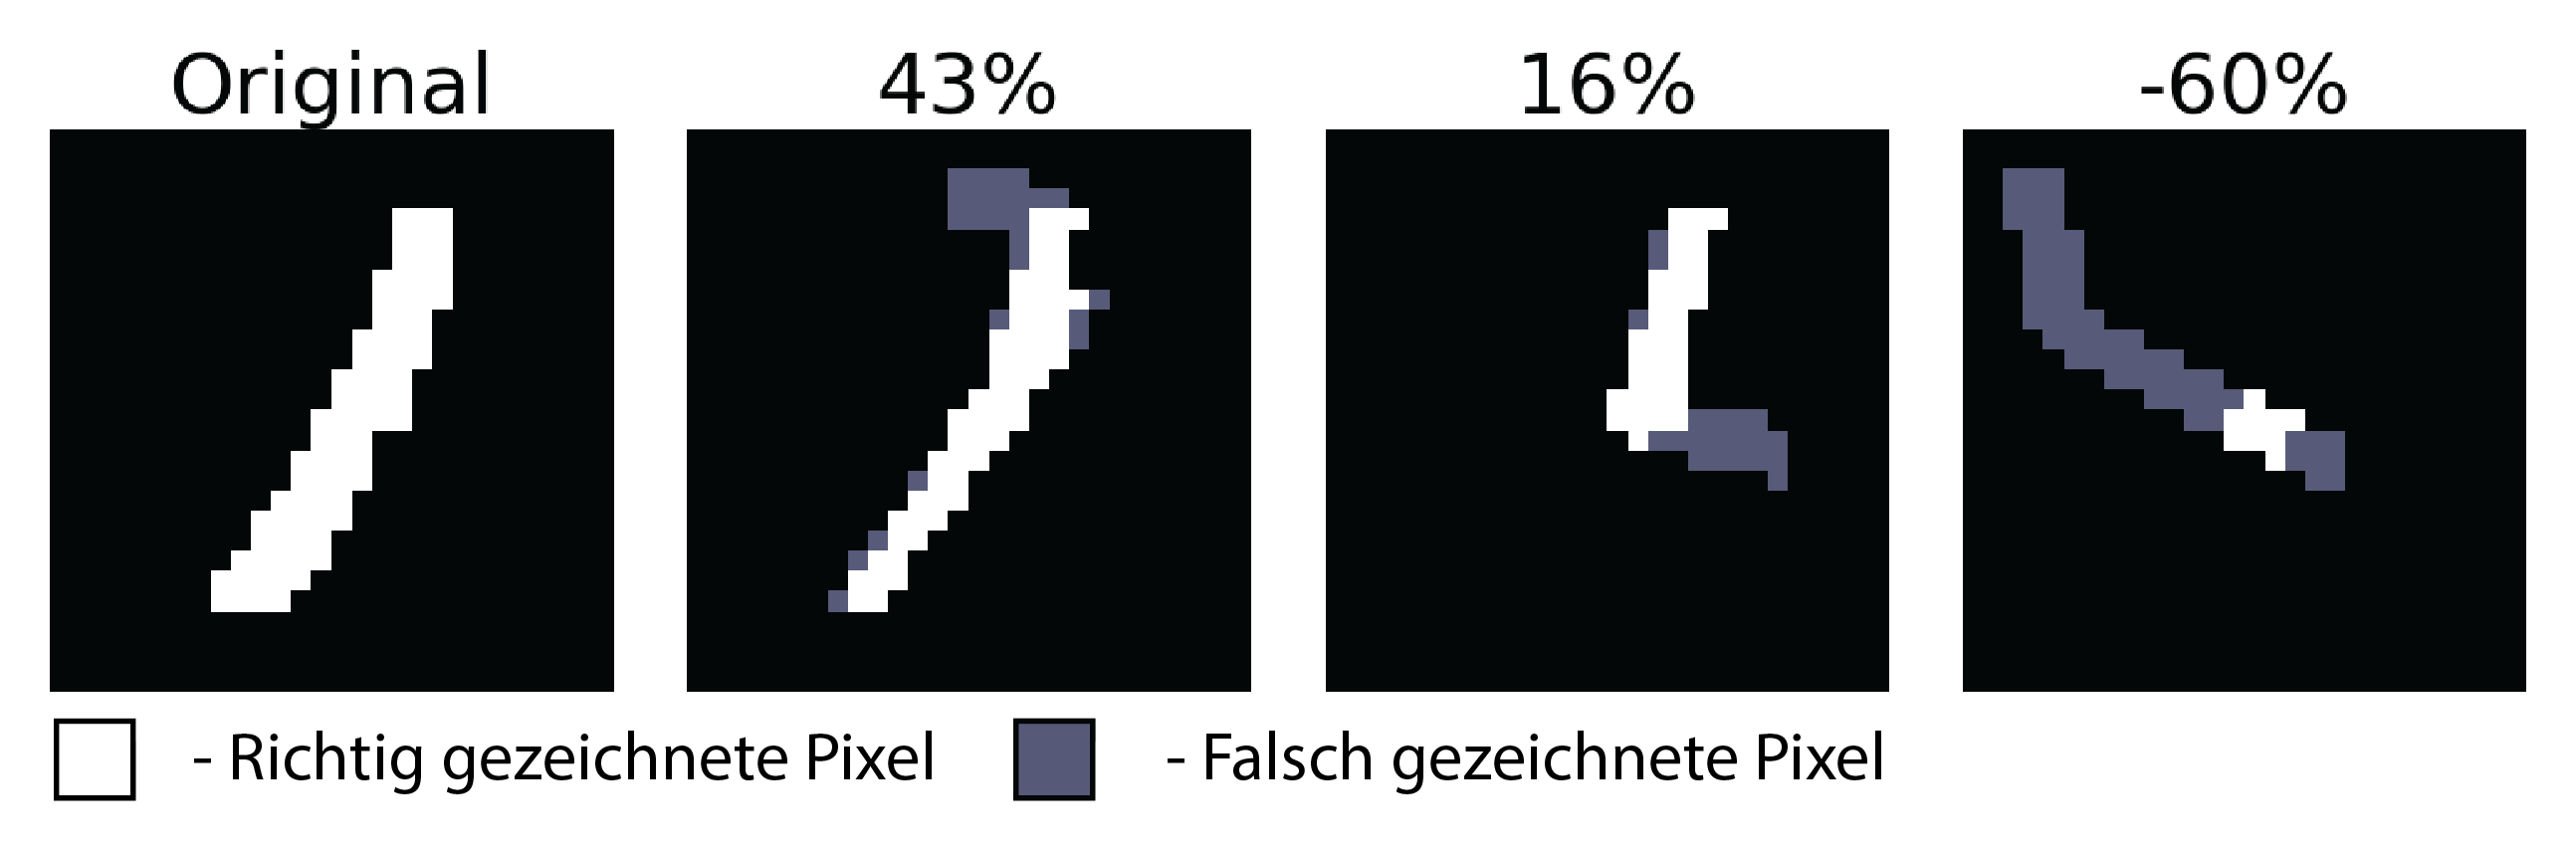
\includegraphics[width=\textwidth]{images/methode/ubereinstimm.png}
 \caption{Drei Beispiele für den Wert des Kriteriums der Übereinstimmung. (eigene Abbildung)}\label{fig:ubereinstimmung}
\end{figure}
 
\subsection{Geschwindigkeit}\label{sub:m_eval_speed} Dieses Kriterium
beschreibt, wie schnell die Zeichnung der KI fertig ist. Der Wert des Kriteriums
entspricht dabei der Anzahl Steps bis zur Fertigstellung. Der Punkt der
Fertigstellung ist dabei bei der letzten zeichnenden Action des Agents
definiert. Falls der Agent sich also nach dem Zeichnen weiterhin
nicht-Zeichnende Actions ausführt, so werden diese nicht mehr zu der Zeichnung
gezählt, weil die Zeichnung nicht beeinflusst wird.

\subsection{Zeichnende Zeit}\label{sub:m_eval_zeichnend} Das Kriterium der
zeichnenden Zeit beschreibt, in wie vielen Steps pro Episode die KI eine
zeichnende Action ausführt. Dieser Wert ist als ein prozentualer Anteil
angegeben und berechnet sich somit aus der Anzahl zeichnender Steps dividiert
durch die Anzahl aller Steps pro Zeichnung.

\subsection{Übermalung}\label{sub:m_eval_uebermalung} Das Kriterium der
Übermalung beschreibt, wie viele Pixel pro zeichnung mehrfach bemalt werden.
Jeder Pixel, auf dem die KI also zwei oder mehr Mal malt, erhöht den Wert dieses
Kriteriums um Eins. Jeder Pixel trägt dabei höchstens einmal zu diesem Kriterium
bei. Das heisst, dass vielfach bemalte Pixel gleich behandelt werden wie
zweimal bemalte Pixel. 

\section{Variationen}\label{chap:m_var} Dieses Unterkapitel beschreibt die
Variationen der KI. Jede Variation erweitert das Grundprogramm (siehe
\doubleref{chap:m_grund}) zu einer funktionalen, nachzeichnenden KI. Die meisten
der Variationen unterscheiden sich dabei hauptsächlich im Fokus auf die
definierten Kriterien (siehe \doubleref{chap:m_eval}). Jede der Variationen
versucht, die Leistung in einem ausgewählten Kriterium zu maximieren. Eine
Anpassung der Reward-Function (siehe \doubleref{sub:t_rl_func}) zielt auf diesen
Effekt ab. Die verschiedenen Variationen sind teilweise untereinander
kombinierbar. Eine der Variationen ist auf kein Kriterium spezialisiert und
versucht stattdessen allgemein das Verhalten der KI zu verbessern.
 
\subsection{Basis Reward-Function}\label{sub:m_var_base} Die Basis
Reward-Function ist die einfachste Erweiterung des Grundprogramms. Diese
Reward-Function implementiert das Kriterium der prozentualen Übereinstimmung
(siehe \doubleref{sub:m_eval_proc}). Der Reward für eine Action berechnet sich
aus der Differenz zwischen der prozentualen Übereinstimmung vor dem Ausführen
der Action und der prozentualen Übereinstimmung nach dem Ausführen der Action
(also $K(t-1)$ und $K(t)$). Somit wird der Reward $R$ zum Step $t$ durch
folgende Formel berechnet.
\[ R(t) = K(t) - K(t-1) \] Der Reward eines Steps entspricht folglich nicht der
gesamten prozentualen Übereinstimmung zu einem Step. Stattdessen entspricht der
Reward der Veränderung der prozentualen Übereinstimmung, ausgelöst durch die
Action in einem Step. Der akkumulierte Reward (siehe \doubleref{sub:t_rl_func})
enstspricht dem absoluten Wert der prozentualen Übereinstimmung. 

Die prozentuale Übereinstimmung ist das grundlegendste Kriterium für die
Tätigkeit des Nachzeichnens und hat ausserdem den Vorteil, dass kleine
Verbesserungen bereits zu einem positiven Reward führen können. Das ist in den
ersten Episoden des Trainings für die KI von entscheidender Bedeutung. Aus
diesem Grund ist die Basis Reward-Function zumindest in ähnlicher Form in allen
anderen Variationen ebenfalls vertreten.

\subsection{Spezialisierung auf Erkennbarkeit}\label{sub:m_var_rec} Das
Kriterium der Erkennbarkeit kann, anders als die anderen Kriterien, nur
teilweise in die Reward-Function integriert werden. Das Kriterium strebt eine
Erkennbarkeit an, die unabhängig von der Art der Strichbilder ist (siehe
\doubleref{sub:m_eval_rec}). Die klassifizierende KI kann allerdings jeweils nur
eine Art von Strichbildern erkennen. Deswegen spezialisiert sich diese Variation
allein auf das Nachzeichnen von Zahlen und verwendet dafür die entsprechende
klassifizierende KI.

Die Variation verwendet die Stopp Action (siehe
\doubleref{sub:m_grund_erweiterungen}). Sobald die nachzeichnende KI die Stopp
Action wählt, überprüft die klassifizierende KI, ob das Bild erkennbar ist. Der
Reward entspricht dabei dem Output des Neurons, welches die Zahl beurteilt, die
nachgezeichnet werden sollte. Dieser Output wird als Reward um $0.8$ verringert.
Der maximale Reward für eine erkennbare Zahl ist somit $1 - 0.8 = 0.2$. Negative
Rewards werden mit einem Faktor von $0.5$ multipliziert, damit die KI nicht zu
hohe negativen Rewards erhält.

\subsection{Spezialisierung auf Geschwindigkeit}\label{sub:m_var_speed} Diese
Variation verwendet die Stopp Action in der Reward-Function um eine möglichst
hohe Geschwindigkeit zu erzielen. Der Reward für die Geschwindigkeit berechnet
sich dabei aus folgendem Prinzip: Umso früher der Agent die Stopp Action
auswählt, desto höher ist der Reward für diese Action. Um zu verhindern, dass
der Agent die Stopp Action direkt im ersten Step wählt, löst die Reward-Function
erst ab einer prozentualen Übereinstimmung von mehr als $80\%$ einen positiven
Reward aus. Ansonsten ist der Reward der Stopp Action negativ. Der Reward über
und unter dieser Schwelle von $80\%$ ist eine statische Zahl. Eine prozentuale
Übereinstimmung von $90\%$ löst also keinen grösseren Reward aus als eine
prozentuale Übereinstimmung von $80\%$. Experimente mit dynamischen Rewards
scheiterten bisher. Ein möglicher Grund dafür ist, dass die KI je nach Situation
zu hohe oder zu niedrige Rewards erhält.

Der Reward wird mit einem Faktor multipliziert, der von der Geschwindigkeit
abhängt. Dieser Faktor ist nicht linear und stattdessen durch die folgende Funktion definiert:
$$ f_{speed} = 1 - (\frac{t}{64})^{3}$$ (Siehe Abbildung Funktion) Dabei ist
$t$ der aktuelle Step und die Zahl $64$ entspricht der maximalen Anzahl Steps,
was somit den Wert der geringsten möglichen Geschwindigkeit ausmacht. Die Kurve
der verwendeten Funktion verhindert, dass der Reward zu schnell abfällt.

\subsection{Spezialisierung auf zeichnende Zeit}
Diese Variation hat zum Ziel, den Wert des Kriteriums der zeichnenden Zeit zu
maximieren. Das heisst, die KI soll sich so wenig wie möglich bewegen ohne dabei
zu zeichnen. Dieser Effekt wird dadurch angestrebt, dass nicht zeichnende
Aktionen einen negativen Reward von $-0.05$ auslösen. Ansonsten unterscheidet
sich die Reward Function von der Basis Reward-Function nicht. Auch diese
Variation verwendet die Stopp Action (spezifisch in Kombination mit der
Spezialisierung auf Geschwindigkeit oder Erkennbarkeit), weil die KI nach einer
gewissen Anzahl Steps keine nützlichen Actions mehr hat und ohne Stopp Action in
diesem Fall unschuldig negative Rewards erhalten würde.

\subsection{Spezialisierung auf keine Übermalung}
Diese Variation versucht, die KI davon abzuhalten, Pixel mehrfach zu übermalen.
Jeder übermalte Pixel senkt dabei den Reward der Basis Reward-Function um einen
definierten Betrag. Pro Action ist allerdings das übermalen von drei Pixeln
erlaubt und somit von negativen Rewards befreit. Diese Variation ist ohne
die Stopp Action verwendbar, kann aber auch mit dieser kombiniert werden.


\subsection{Physikalische Umgebung}\label{sub:m_var_phy} Diese Variation
spezialisiert sich auf kein Kriterium. Stattdessen verändert sie die Umgebung,
sowie auch den Input und den Output des neuronalen Netzes (siehe
\doubleref{sub:t_rl_func}). Durch diese Veränderungen löst sich die Variation vom
Grundprogramm.
 
Die Variation ergänzt die Umgebung durch physikalische Simulationen. Der Agent
hat neu eine Geschwindigkeit, die durch einen Vektor $\vec{v}$ dargestellt ist.
Die Geschwindigkeit beschreibt, um wie viele Pixel und in welche Richtung sich
der Agent pro Step bewegt. Die folgende Formel beschreibt, wie sich die Position
des Agenten vom Step $t$ bis zum nächsten Step $t+1$ verändert:
\[ \vec{p}(t+1) = \vec{p}(t) + \vec{v}(t) \]
$\vec{p}(t)$ beschreibt die Position des Agents als einen Ortsvektor auf der
Zeichenfläche zum Step $t$ und $\vec{v}(t)$ beschreibt die Geschwindigkeit des
Agenten zum Step $t$. Die Position rundet in jedem Step auf ganze Zahlen. Das
kommt daher, dass die Geschwindigkeit auch Dezimalzahlen annehmen kann, aber die
Position nur durch ganze Zahlen dargestellt ist.
 
Zur Geschwindigkeit des Agents wird in jedem Step ein Beschleunigungsvektor
addiert. Jede Action, die der Agent wählen kann, entspricht einem anderen
Beschleunigungsvektor. Der Action-Space (siehe \doubleref{sub:t_rl_func})
besteht neu aus $42$ Actions. $21$ der $42$ Actions beschreiben
Beschleunigungsvektoren im zeichnenden Zustand. Die anderen $21$ Actions
beschreiben dieselben Vektoren im nicht zeichnenden Zustand. Die 21
verschiedenen Beschleunigungsvektoren im Actions-Space sind in der folgenden
Formation angeordnet: (siehe \autoref{fig:physics-actionspace}).
 
%bild physik actionspace
\begin{figure}[!ht]
 \centering
 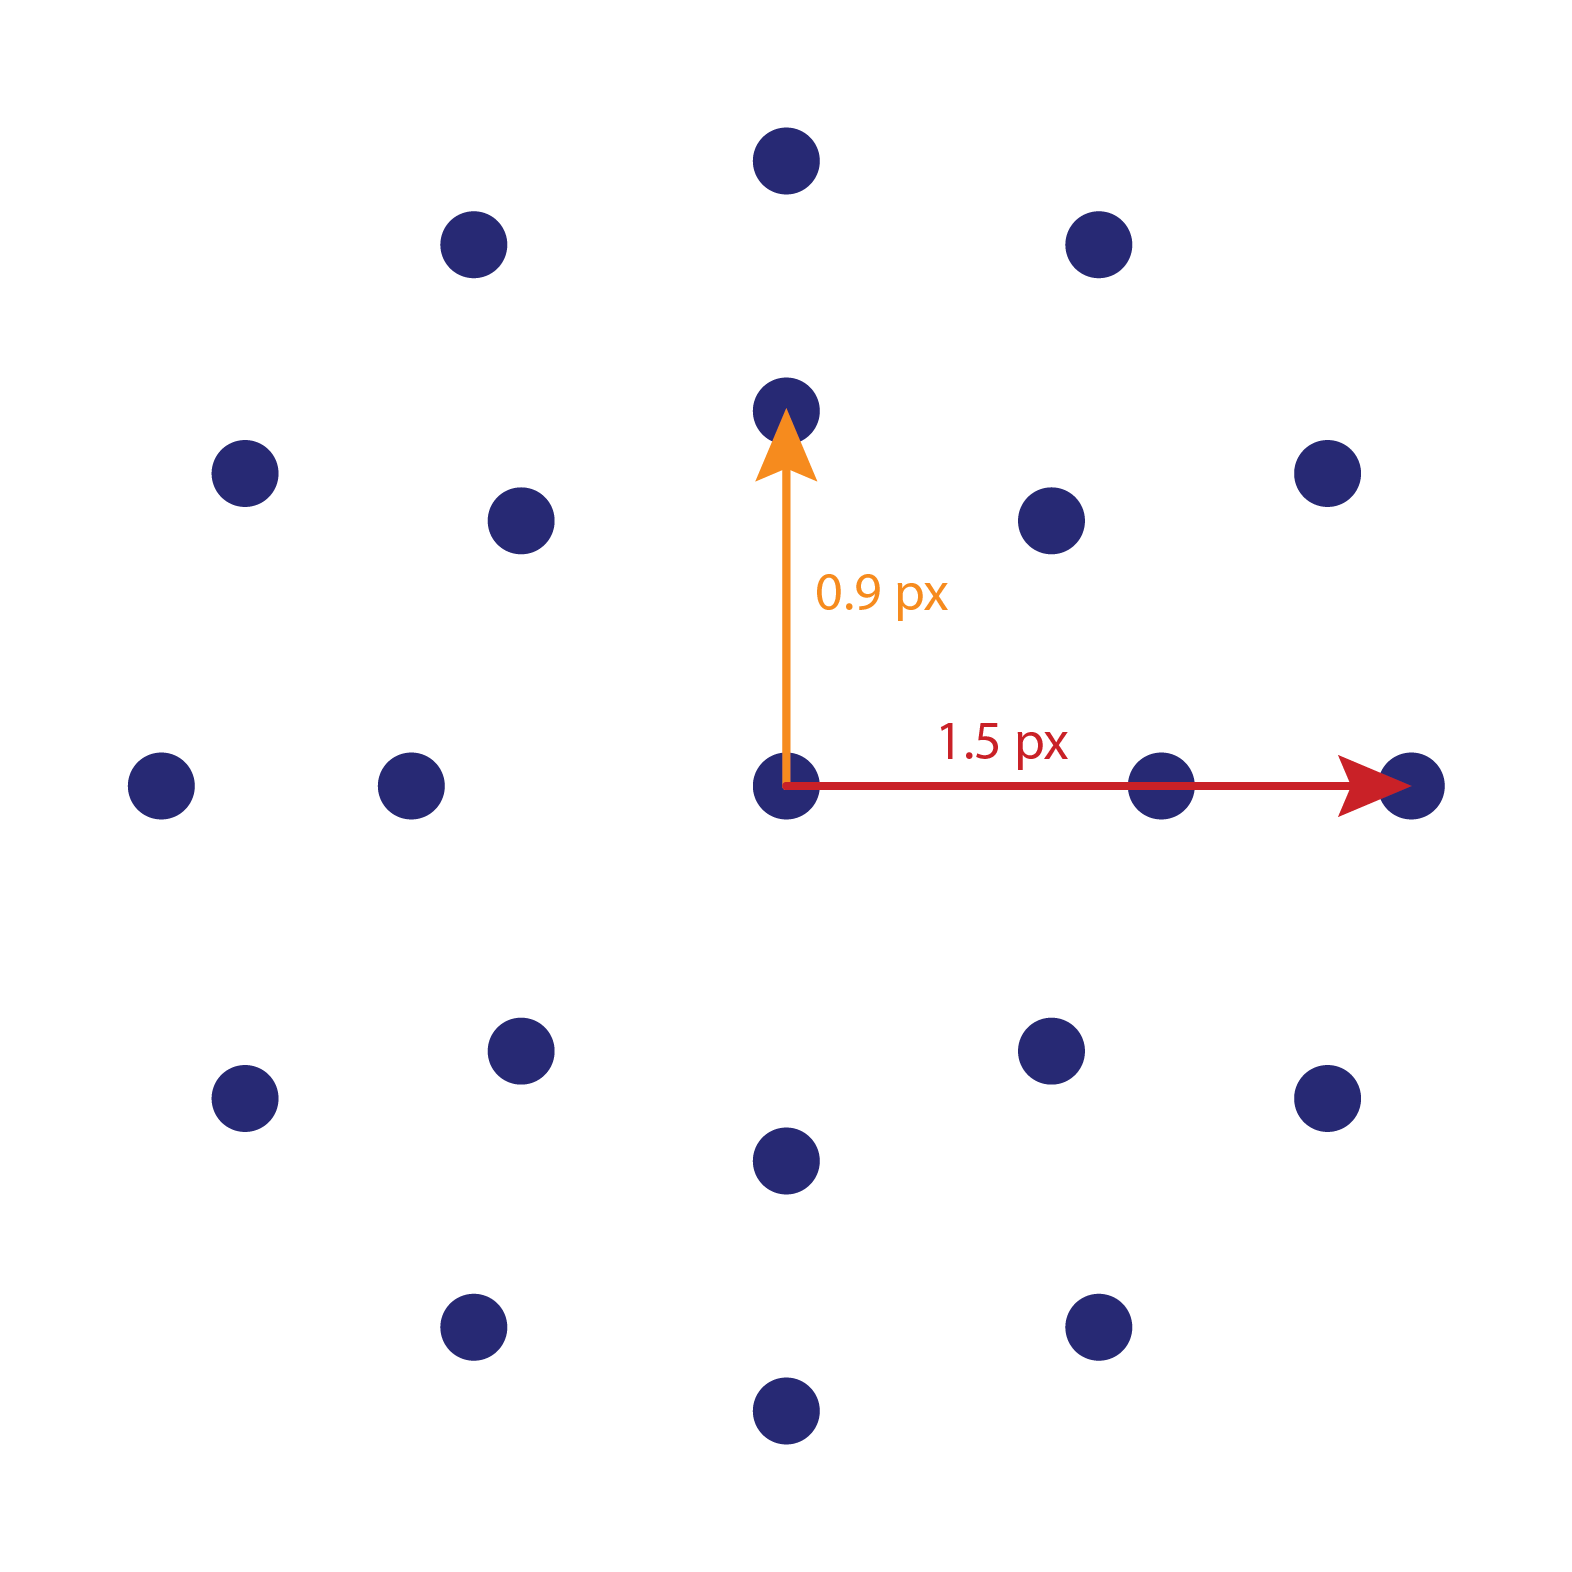
\includegraphics[width=\textwidth-6cm]{images/methode/physics-actionspace.png}
 \caption{Action-Space in der physikalischen Umgebung. (eigene Abbildung)}\label{fig:physics-actionspace}
\end{figure}
 
 
Mit dem gewählten Beschleunigungsvektor $\vec{a}(t)$ berechnet sich die
Geschwindigkeit im nächsten Step $t+1$ aus dem aktuellen Step $t$ durch folgende
Formel:
\[ \vec{v}(t+1) = \vec{v}(t) + \vec{a}(t) \] Der Betrag der Geschwindigkeit
$\vec{v}(t+1)$ des Agents wird in jedem Step, unabhängig von der gewählten
Action, um $0.3$ Pixel pro Step verringert. Das simuliert eine Reibungskraft,
die auf den Agent einwirkt.

Um die Geschwindigkeit des Agents in die Observation (siehe
\doubleref{sub:t_rl_func}) zu integrieren, wird der Local image Patch (siehe
\doubleref{sub:t_ver_dood}) verschoben. Im Grundprogramm entspricht der
Mittelpunkt des Local image Patches genau der Position des Agents. Neu befindet
sich der Mittelpunkt dort, wo sich der Agent laut seiner aktuellen
Geschwindigkeit im nächsten Step befinden wird. Durch diese Verschiebung des
Local image Patches erhält der Agent Informationen über seine Geschwindigkeit,
ohne dessen numerischen Wert zu kennen. Wie im Grundprogramm gibt der Local
image Patch den gesamten Bereich an, in dem sich der Agent im nächsten Step
befinden kann. Die tatsächliche neue Position des Agents wird durch die Action
seiner Wahl bestimmt. Die Grösse des Local image Patches schrumpft von
$7\times7$ Pixeln auf $5\times5$ Pixel, da alle möglichen Positionen des Agents
nach einem Step auf einem $5\times5$ Feld Platz haben (siehe
\autoref{fig:patch-move}).
 
%bild local patch verschiebung
\begin{figure}[!ht]
 \centering
 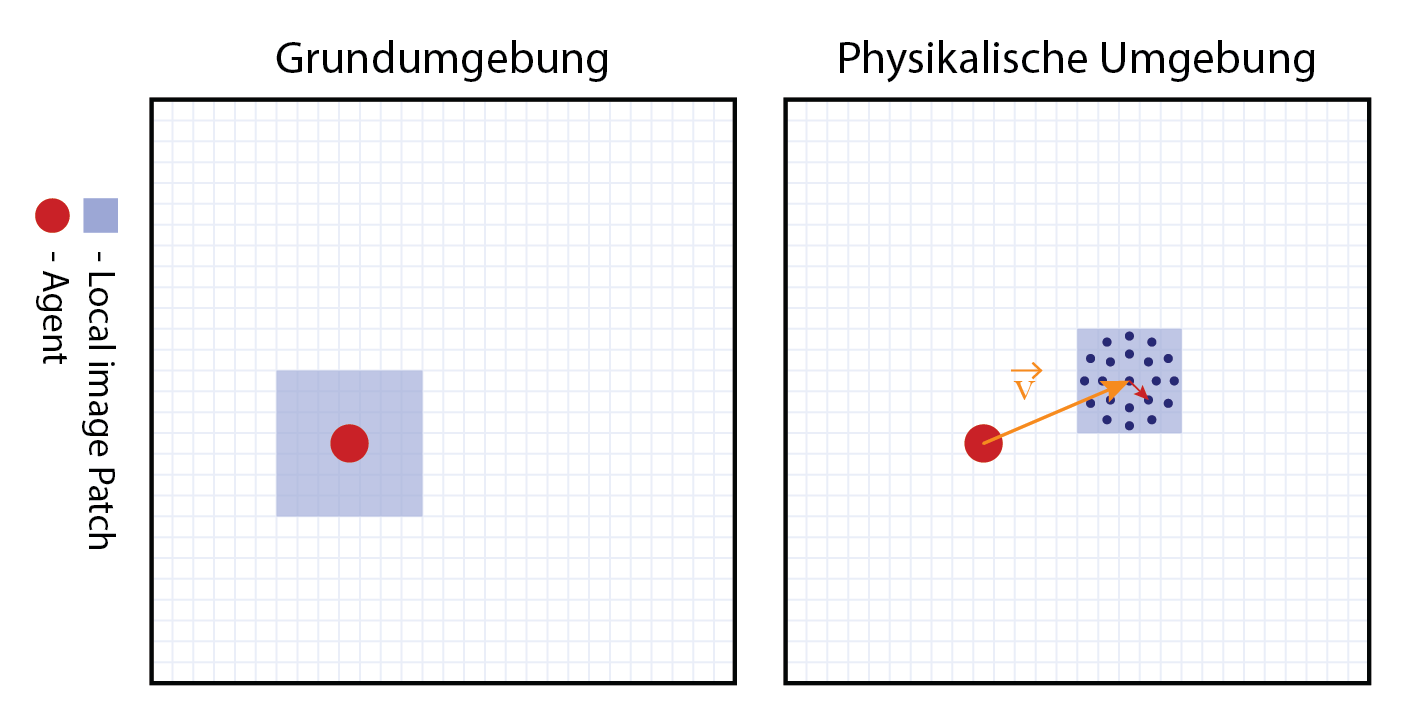
\includegraphics[width=\textwidth]{images/methode/patch-move.png}
 \caption{Angabe der Geschwindigkeit durch eine Verschiebung des Local image Patches. (eigene Abbildung)}\label{fig:patch-move}
\end{figure}
 
Ein weiteres Problem ist, dass der Agent sich durch seine Geschwindigkeit aus
den vorgegebenen Grenzen der Zeichenfläche begeben kann. Im Grundprogramm 
(siehe \doubleref{sub:m_grund_dood}) kann der Agent Actions, die ihn in eine
unzulässige Position bewegen würden, nicht auswählen. Wenn allerdings in der
physikalischen Umgebung die Geschwindigkeit des Agents zu hoch ist, kann dieser
keine Actions mehr wählen, die ihn innerhalb der Grenzen der Zeichenflächen
halten würden. Als Lösung wird diesen Fällen die Geschwindigkeit des Agents auf den
Nullvektor zurückgesetzt und die Reward-Function löst einen negativen Reward von
$-0.05$ aus.

\section{Generative Zeichner}\label{chap:m_gen} Die generativen Zeichner sind
eine Gruppe an Variationen der KI, die sich von der Aufgabe des Nachzeichnens
entfernen. Trotzdem basieren auch diese Versionen auf dem Grundprogramm (siehe
\doubleref{chap:m_grund}) und verändern dieses kaum. Die Aufgabe der generativen
Zeichner lautet, Motive ohne eine Vorlage zu zeichnen. So soll die KI nach dem
Training mit einem bestimmten Motiv eigene Zeichnungen von diesem Motiv
erstellen können. Beispielsweise soll die generative KI (also ein generativer
Zeichner) auf das Zeichnen der Zahl Zwei trainiert werden, damit diese nach dem
Training ohne eine Vorlage eine Zwei zeichnen kann.

\subsection{Trainingsstrategie}\label{chap:m_gen_train} Die Strategie des
Trainings für die generative KI unterscheidet sich von derjenigen der
nachzeichnenden KI stark, da die nachzeichnende KI nach dem Training ohne
Vorlage nichts zeichnet.

Die Trainingsstrategie der generativen KI funktioniert folgendermassen: Im Input
Channel des neuronalen Netzes (siehe \doubleref{sub:t_ml_nn}), wo der
nachzeichnenden KI das Bild der Vorlage gegeben wird, hat die generative KI ein
vollkommen schwarzes Bild (Alle Werte der Bitmap sind $0$). Der Channel für die
Vorlage wird nicht entfernt, weil während dem Training der generativen KI zu
einem gewissen Anteil trotz dessen Aufgabe eine Vorlage gegeben wird. Die
Wahrscheinlichkeit, dass für eine Episode der KI eine Vorlage gezeigt wird,
sinkt dabei linear über das Training hinweg von $1$ auf $0.25$. Zu Beginn des
Trainings unterscheidet sich die generative KI somit nicht von der
nachzeichnenden KI. Erst nachdem die generative KI das Nachzeichnen weitgehend
erlernt hat, erlernt diese ihre eigentliche Aufgabe, indem sie zunehmend
seltener eine Vorlage erhält. die generative KI trainiert insgesamt für $6'000$
Episoden

Die generative KI verwendet die Basis Reward-Function (siehe
\doubleref{sub:m_var_base}) unabhängig davon, ob in der aktuellen Episode eine
Vorlage gezeigt wird oder nicht. Da die Basis Reward-Function eine Vorlage
benötigt, mit der die Zeichnung verglichen werden kann, hat die generative KI
während dem Training im Hintergrund immer eine Vorlage. Das bedeutet, dass wenn
dem neuronalen Netz der generativen KI keine Vorlage gezeigt wird, so hat die
Reward-Function trotzdem eine Vorlage als Vergleich zu der Zeichnung.
Prinzipiell ist ein generativer Zeichner während dem Training also ein blinder
Nachzeichner. Der relevantere Reward für die generative KI basiert allerdings
nicht auf auf dem Kriterium der prozentualen Übereinstimmung, welches die Basis
Reward-Function verwendet, sondern auf dem Kriterium der Erkennbarkeit (siehe
\doubleref{sub:m_eval_rec}). Da ein generativer Zeichner ein Motiv ohne weitere
Spezifikationen zeichnen soll, ist die Erkennbarkeit des Motives von grösster
Priorität. Die generative KI verwendet deswegen neben der Basis Reward-Function
ebenfalls die auf Erkennbarkeit spezialisierte Reward-Function (siehe
\doubleref{sub:m_var_rec}). 

Anders als die nachzeichnende KI, startet die generative KI für jede Zeichnung
am selben vordefinierten Ort. Das verringert den Trainingsaufwand, aber bedeutet
auch, dass nach dem Training die KI nur eine einzige Ausgangslage kennt. Nach
dem Training ist die Wahl der Actions deterministsch, Da die KI stets die Action
mit dem höchsten Q-Value wählt (siehe \doubleref{chap:m_auswert}). Zusammen mit
der unveränderlichen Ausgangslage führt der Determinismus dazu, dass die KI nur
eine einzige Zeichnung produzieren kann. 


%Todo: In diskussion einfügen
Diskussion Gedanken
(Generierer nur möglich mit nachzeichner)
(Prozess des Nachzeichnens entscheidend für Generierer)


\subsection{Nicht deterministische Zeichnungen}\label{chap:m_gen_det} Damit die
generative KI unterschiedliche Bilder zeichnet und nicht deterministisch ist,
benötigt der Zeichenprozess ein Element von Zufall. Es gibt verschiedene Ansätze
um diesen Zufall zu integrieren.

Der erste Ansatz ist, nach dem Training der generativen KI die Softmax Policy
zur Wahl der Actions zu verwenden (siehe \doubleref{sub:t_rl_func}). Die Softmax
Policy macht die Wahl der Action in jedem Step vom Zufall abhängig. Ausserdem
hat die Softmax Policy gegenüber von Epsilon-Greedy den Vorteil, dass Actions
nie komplett vom Zufall bestimmt werden, sondern nach einer bestimmten
Wahrscheinlichkeitsverteilung gewählt werden. Als weiterer Vorteil ist die
Wahrscheinlichkeitsverteilung durch die Softmax Temperatur variierbar. Diese
Eigenschaft ist für den Erfolg der Softmax Policy als Lösung für das Problem der
deterministischen Zeichnungen entscheidend, weil die KI nur mit einer geringen
Freiheit in der Wahl der Actions umgehen kann: Eine einzige falsche Action kann
bereits dazu führen, dass das Motiv der Zeichnung nicht mehr erkennbar ist. Eine
tiefe Softmax Temperatur, in einem Intervall zwischen $0.03$ und $0.01$,
versichert, dass Actions mit einem geringen Q-Value nur in seltenen Fällen
gewählt werden.

Trotz geringer Softmax Temperatur ist die Freiheit in der Wahl der Actions zu
gross und führt dazu, dass die generative KI häufig keine erkennbaren Bilder
produziert. Eine Weiterführung des ersten Ansatz ist deshalb die Beschränkung
der Wahl auf die $5$ Actions mit der höchsten Wahrscheinlichkeit. Diese
Weiterführung hat mehr Erfolg als der erste Ansatz, weil Actions mit einer
tiefen Wahrscheinlichkeit gar nicht mehr ausgeführt werden können. Ansonsten
würde fast in jeder Zeichnung mindestens eine unwahrscheinliche Action
ausgeführt werden.

Die nachzeichnende KI verwendet standardmässig Epsilon-Greedy anstelle der
Softmax-Policy, weil die Leistung in allen Kriterien ohne die Softmax Activation
deutlich höher ist. Wird allerdings wie im ersten Ansatz nach dem Training die
Softmax Policy verwendet, so sollte die KI auch mit der Softmax Policy
trainieren. Die Softmax Temperatur ist während dem Training statisch als $0.05$
definiert. Eine dynamische Anpassung der Softmax Temperatur während dem Training
beeinflusst das Verhalten der KI nicht bemerkbar.

Der zweite Ansatz ist, den Input in das neuronale Netz auf zufällige Weise
anzupassen, da ein unterschiedlicher Input zu unterschiedlichen Beurteilungen
führt. Eine Möglichkeit, um den Zufall zu integrieren, liegt im Channel des
Inputs in das neuronale Netz, wo der KI eine Vorlage gezeigt wird. Der
generativen KI wird generell ein in diesem Channel ein schwarzes Bild anstelle
einer Vorlage gezeigt. Werden die Werte der Pixel dieses schwarzen Bildes mit
zufälligen Werten zwischen $0$ und $1$ ersetzt, so verändert sich der Input in
das neuronale Netz und somit auch der Output. Die KI trifft also Entscheidungen,
die von zufälligen Werten abhängen. Damit dieser Ansatz funktioniert, muss
bereits während dem Training diese Zufallsquelle integriert werden.

%Todo: Änderung der Startposition
%Todo: Mehr Text

\section{Auswertung}\label{chap:m_auswert}
Die Auswertung beschreibt das sammeln der Leistungsdaten der verschiedenen
Variationen und Versionen der KI. Diese Daten machen das Resultat der Methode
aus. Die Leistungsdaten beruhen auf den objektiven Werten der definierten
Kriterien (siehe \doubleref{chap:m_eval}). Die Auswertung wird für die
Variationen der nachzeichnenden KI und die Variationen der generativen KI
separat beschrieben, da diese sich in den beiden Fällen unterscheidet.

\subsection{Auswertung der nachzeichnenden KI}\label{chap:m_auswert_nachzeich}
Die Variationen der nachzeichnenden KI werden auf ihre Leistung für drei
verschiedene Datensets geprüft. Die drei Datensets enthalten verschiedene Arten
von Strichbildern und jeweils eine klassifizerende KI, welche die spezifischen
Strichbilder erkennen kann (siehe \autoref{tab:models}). Im Falle des QuickDraw
Datensets wird die KI allerdings nur auf das Nachzeichnen von zehn Motiven
überprüft. Die zehn Motive sind: `Amboss', `Apfel', `Besen', `Eimer',
`Bulldozer', `Uhr', `Wolke', `Computer', `Auge' und `Blume' (siehe
\autoref{fig:quickdraw-examples}). Die Bilder in den drei Datensets werden im
Training nicht verwendet, sind aber gleich verarbeitet wie die Trainingsdaten
(siehe \doubleref{sub:m_grund_data}).

%Bild images dataset
\begin{figure}[!ht]
    \centering
    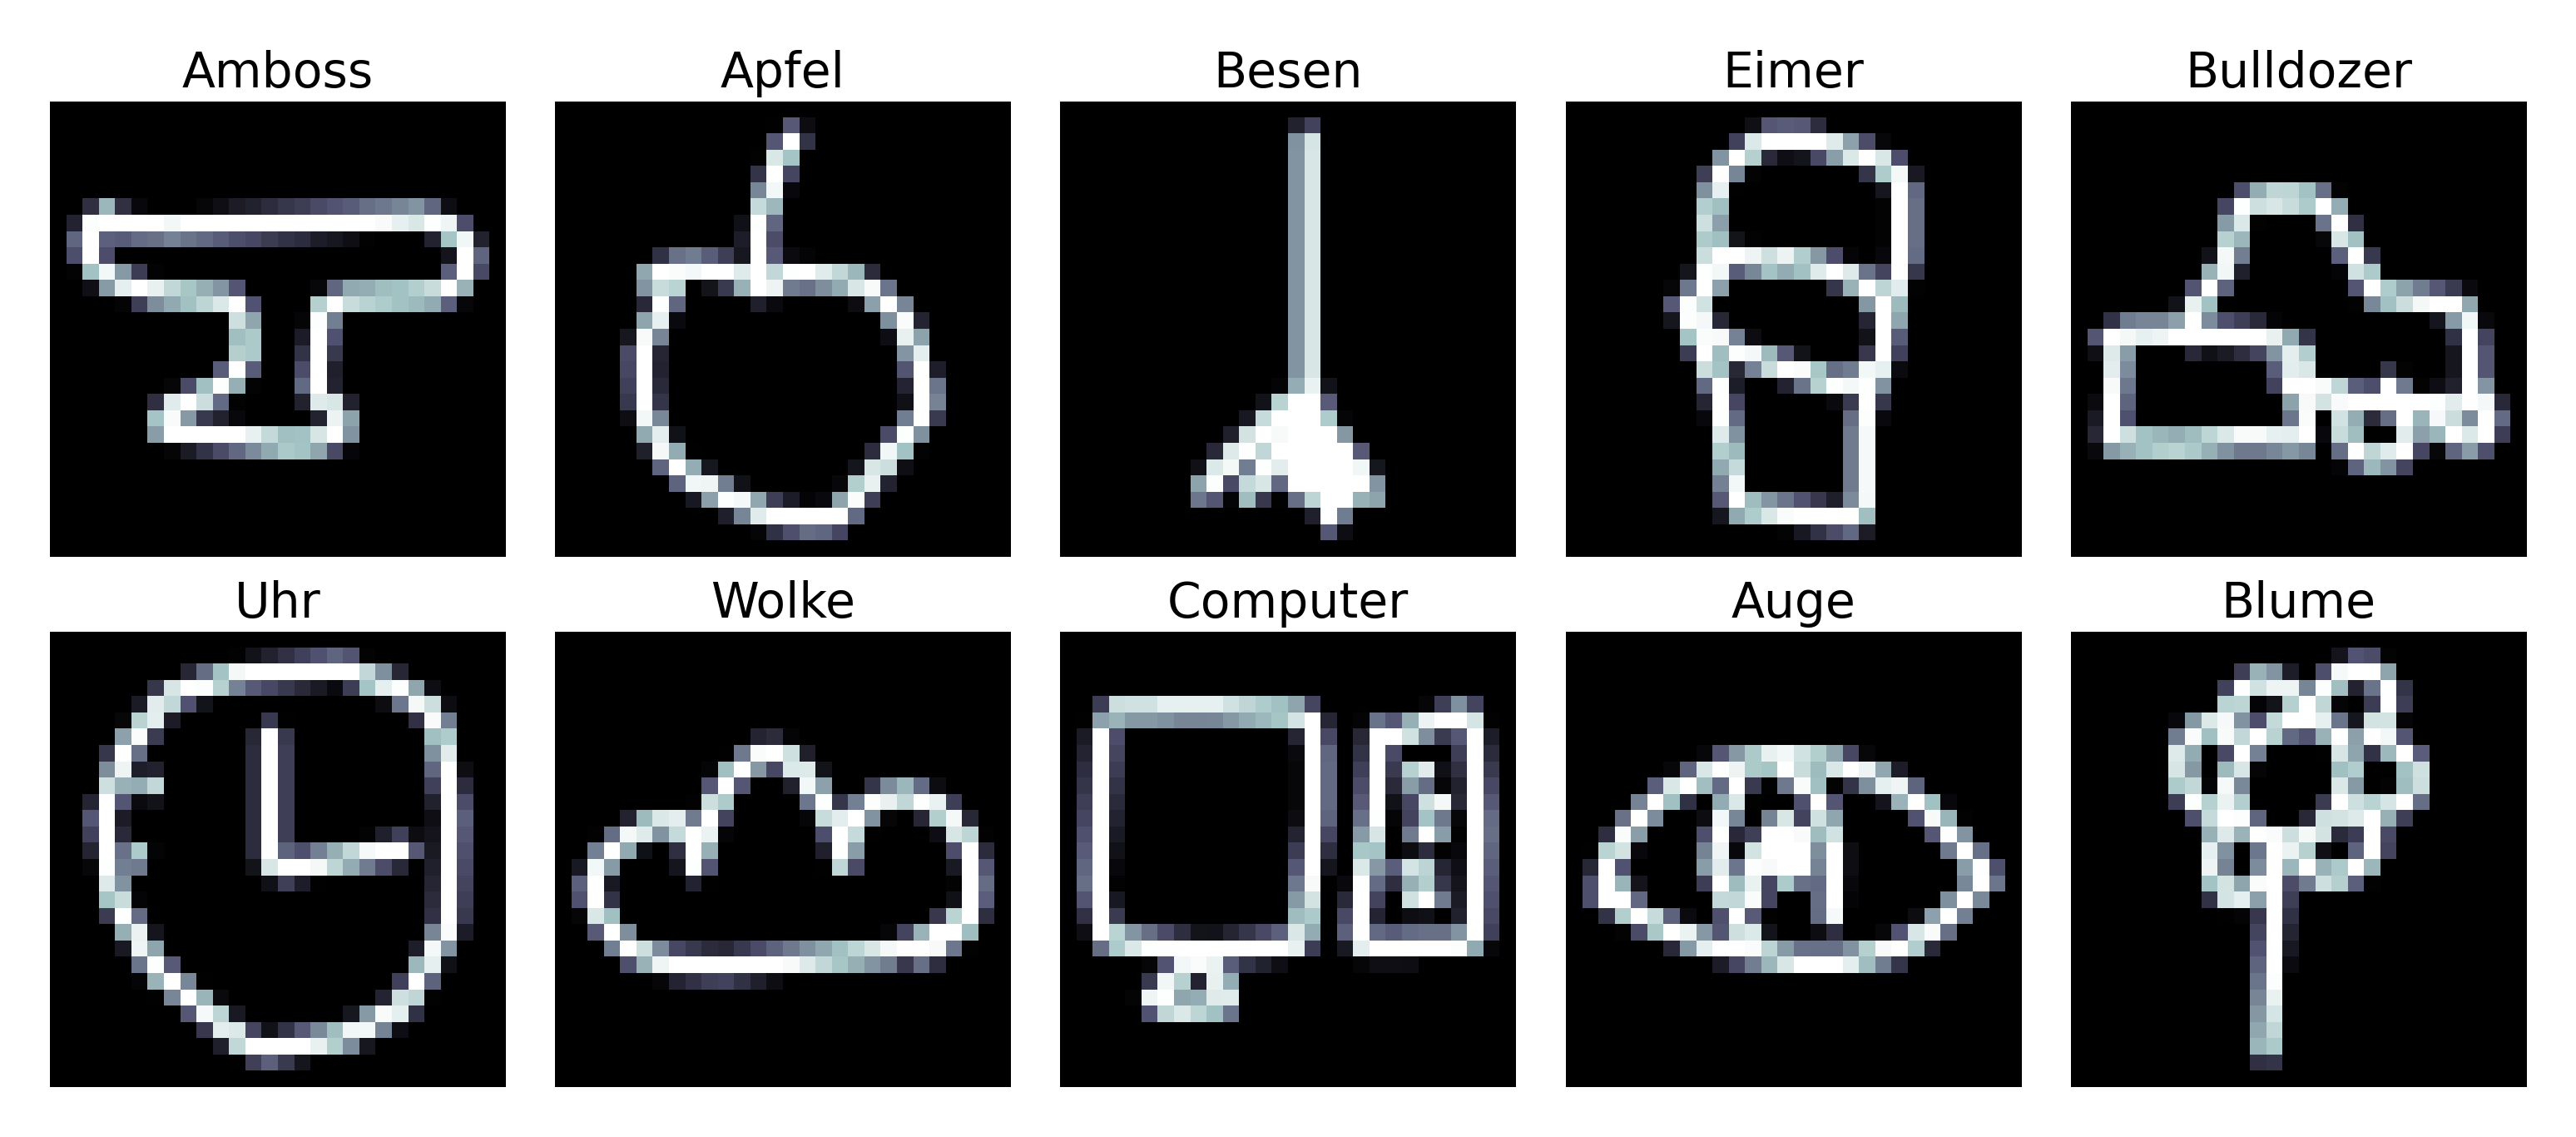
\includegraphics[width=\textwidth]{images/methode/quickdraw-examples.png}
    \caption{Beispiele der verwendeten Motive aus dem QuickDraw Datenset. (eigene Abbildung)}\label{fig:quickdraw-examples}
\end{figure}

Eine Testumgebung erfasst die Leistung der KI (siehe \doubleref{sub:t_ml_func}).
Zwischen der Trainingsumgebung und der Testumgebung sind zwei relevante
Unterschiede. Erstens trainiert die KI in der Testumgebung nicht. Die
Testumgebung übernimmt eine trainierte Version der nachzeichnenden KI und
verändert diese während dem Test nicht. Zweitens wählt der Agent Die Actions
deterministisch. In jedem Step wird die Action mit dem höchsten Q-Value gewählt.

Im Test zeichnet die KI $2'000$ Strichbilder nach. Am Ende jeder Zeichnung wird
der Zahlenwert der verschiedenen Kriterien (siehe \doubleref{chap:m_eval}) ihrer
Definition entsprechend berechnet und gespeichert. Der Durchschnitt aller
gespeicherten Werte eines Kriteriums entspricht der Leistung der KI in diesem
Kriterium. Da das Kriterium der Erkennbarkeit entweder den Wert $0$ oder $1$
hat, ergibt der Durchschnitt aus allen Werten dieses Kriteriums eine prozentuale
Angabe (in Dezimalform) darüber, in wie vielen Fällen das richtige Motiv erkannt
wird.

\subsection{Auswertung der generativen Zeichner}\label{chap:m_auswert_gen}

Die Variationen der generativen KI werden auf ihre Leistung in dem Kriterium der
Erkennbarkeit, der Geschwindigkeit und der zeichnenden Zeit geprüft (siehe
\doubleref{chap:m_eval}). Die übrigen Kriterien ergeben ohne eine
nachzuzeichnende Vorlage keinen Sinn. Anders als im Training wird der
generativen KI in der Testumgebung in keinem Fall eine Vorlage gezeigt. Die
Startposition ist auf die selbe vordefinierten Position wie im Training gesetzt.
Die Wahl der Actions ist nicht deterministisch, weil die KI in diesem Fall nur
eine einzige Zeichnung produzieren könnte. Stattdessen unterliegt die Wahl der
Actions den selben Zufallselementen (siehe \doubleref{sub:m_gen_det}) wie im
Training der jeweils getesteten Variation.

Im Test generiert die KI 500 Bilder. Das Motiv der Bilder hängt dabei davon ab,
worauf die Variation trainiert ist. Eine Variation wird auf fünf verschiedene
Motive trainiert und anschliessend getestet. Die drei Motive sind: eine Null,
eine Zwei, eine Acht, ein F und eine Blume aus dem QuickDraw Datenset (siehe
\autoref{fig:generative_motives}). Wenn eine Variation im Test die Softmax
Policy verwendet (siehe \doubleref{sub:t_rl_func}), dann ist die Softmax
Temperatur unabhängig von derjenigen im Training bestimmbar. Die Softmax
Temperatur beeinflusst dabei wie viel Varianz in den Zeichnungen ist.

%Todo Abbildung Null, Zwei, Acht, F, Bluem
%\label{fig:generative_motives}

Wie im Test der nachzeichnenden KI (siehe \doubleref{chap:m_auswert_nachzeich}),
entspricht die Leistung einer Variation dem Durchschnitt der Werte in den
verwendeten Kriterien nach jeder Zeichnung.

